\newpage 
\section[Continuity]{\hyperlink{toc}{Continuity}}

\subsection{Limits and Continuity}
\begin{definition}{Limits}{4.1}
    Let $X, Y$ be metric spaces. Let $E \subset X$, and let $f: E \mapsto Y$. Let $p \in X$ be a limit point of $E$. Then, we say that $\lim_{x\rightarrow p} f(x) = q$ or $f(x) \rightarrow q$ as $x \rightarrow p$ if there exists $q \in Y$ such that for all $\e > 0$, there exists $\delta > 0$ such that for all $x \in E$ with $0 < d_X(x, p) < \delta$ we have that $d_Y(f(x), q) < \e$. 
\end{definition}
\begin{figure}[htbp]
    \centering
    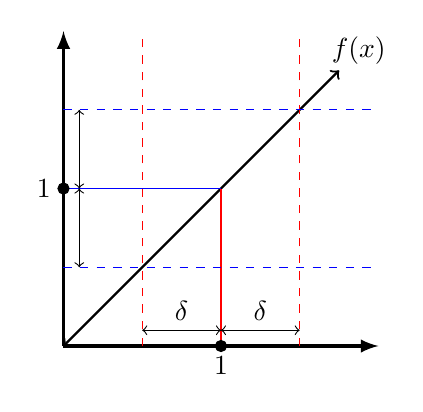
\begin{tikzpicture}[scale=2]
        \draw[-latex,very thick] (0,0)--(2,0);
        \draw[-latex,very thick] (0,0)--(0,2);
        \draw[<->, thick] (0, 0) -- (1.75, 1.75);
        \draw[color = red] (1, 0) -- (1, 1);
        \draw[color = red, dashed] (0.5, 0) -- (0.5, 2);
        \draw[color = red, dashed] (1.5, 0) -- (1.5, 2);
        \draw[<->] (0.5, 0.1) -- (1, 0.1);
        \node[above] at (0.75, 0.1) {$\delta$};
        \draw[<->] (1, 0.1) -- (1.5, 0.1);
        \node[above] at (1.25, 0.1) {$\delta$};
        \draw[color = blue] (0, 1) -- (1, 1);
        \draw[color = blue, dashed] (0, 0.5) -- (2, 0.5);
        \draw[color = blue, dashed] (0, 1.5) -- (2, 1.5);
        \draw[<->] (0.1, 0.5) -- (0.1, 1);
        \node[right] at (0.1, 0.75) {$\e$};
        \draw[<->] (0.1, 1) -- (0.1, 1.5);
        \node[right] at (0.1, 1.25) {$\e$};
        \draw[fill = black] (0, 1) circle (1pt);
        \node[xshift = -0.25cm] at (0, 1) {$1$};
        \draw[fill = black] (1, 0) circle (1pt);
        \node[yshift = -0.25cm] at (1, 0) {$1$};
        \node[yshift = 0.25cm, xshift = 0.25cm] at (1.75, 1.75) {$f(x)$};
    \end{tikzpicture}
    \caption{Visualization of the limit $\lim_{x \rightarrow 1}f(x) = 1$ for $f(x) = x$. For any $\e > 0$, we can take $\delta = \e$ and then we have that $\abs{f(x) - 1} < \e$ if $\abs{x - 1} < \delta$.}
    \label{fig17}
\end{figure}
Note in the above definition that we do not care about $f(p)$, that is, the actual value of $f$ at $p$. In particular, if $p \notin E$, then $f(p)$ is not even necessarily defined. This distinction between the limit and the actual value of a function at a point becomes crucial later on when we want to define a derivative. Although we will discuss this in more detail in Chapter 5, the definition of a derivative of a function $g$ at a point $p \in \RR$ involves the function $f: \RR \rightarrow \RR$ such that:
\begin{align*}
    f(x) = \frac{g(x) - g(p)}{x - p}
\end{align*}
Evidently, the domain of $f$ does not contain the point $p$, but we are interested in the value of $f$ in the limit of $x \rightarrow p$ (which, if it exists, is the value of the derivative).

\begin{figure}[htbp]
    \centering
    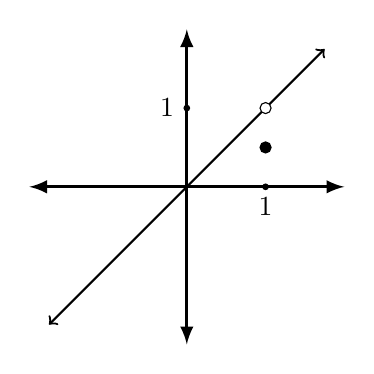
\begin{tikzpicture}
        \draw[latex-latex,very thick] (-2,0)--(2,0);
        \draw[latex-latex,very thick] (0,-2)--(0,2);
        \draw[<->, thick] (-1.75, -1.75) -- (1.75, 1.75);
        \draw[fill = black] (0, 1) circle (1pt);
        \node[xshift = -0.25cm] at (0, 1) {$1$};
        \draw[fill = black] (1, 0) circle (1pt);
        \node[yshift = -0.25cm] at (1, 0) {$1$};
        \draw[fill = white] (1, 1) circle (2pt);
        \draw[fill = black] (1, 0.5) circle (2pt);
    \end{tikzpicture}
    
    \caption{Visualization of the function $f(x) = x$ for $x \in \RR \setminus \set{1}$, $f(x) = 0$ for $x = 1$. In this case, we have that $f(1) = 0$ but $\lim_{x \rightarrow 1} f(x) = 1$, demonstrating that the actual value of the function is irrelevant when defining the limit.}
    \label{fig18}
\end{figure}

\begin{theorem}{}{4.2}
    Let $X, Y$ be metric spaces. Let $E \subset X$ and $f:E \mapsto Y$. Suppose that for all sequences $\set{p_n} \subset E$ with $p_n \rightarrow p$ and $p_n \neq p$, we have that $f(p_n) \rightarrow q \in Y$. Then, this is equivalent to saying that $\lim_{x \rightarrow p} f(x) = q$.
\end{theorem}
\begin{nproof}
    \boxed{\implies} Suppose that $\lim_{x \rightarrow p} f(x) = q$, and let $\set{p_n}$ be a sequence in $E$ with $p_n \rightarrow p$ and $p_n \neq p$ for all $n$. We wish to show that $f(p_n) \rightarrow q$. Let $\e > 0$. We show that there exists $N \in \NN$ such that $d_Y(f(p_n), q) < \e$ for all $n \geq N$. Since $\lim_{x \rightarrow p} f(x) = q$, there exists $\delta > 0$ such that for all $x \in E$ with $d_X(p, x) < \delta$, $d_Y(f(x),q) < \e$. Since we know that $p_n \rightarrow p$, there exists some $N$ such that $0 < d(p_n, p) < \delta$ for all $n \geq N$, so we have that $d_Y(f(p_n), q) < \e$ as required. 

    \boxed{\impliedby} We show the contrapositive. Suppose that $\lim_{x \rightarrow p} f(x) \neq q$. We wish to find a sequence $\set{p_n} \subset E$ with $p_n \rightarrow p$ and $p_n \neq p$ for all $n$ such that $f(p_n)$ does not converge to $q$. Since $\lim_{x \rightarrow p} f(x) \neq q$, then there exists $\e > 0$ such that for all $\delta > 0$, there exists $x \in E$ such that $0 < d_X(x, p) < \delta$ but $d_Y(f(x), q) \geq \e$. For each $\delta$ of the form $\frac{1}{n}$, let $p_n \in E$ be the corresponding value of $x$. Then, $p_n \rightarrow p$, $p_n \neq p$ for all $n$, and $f(p_n)$ does not converge to $q$ as $d(f(p_n), q) \geq \e$ for all $n$. \qed
\end{nproof}

\stepcounter{rudin}

\begin{theorem}{}{4.4}
    When $Y = \CC$ (i.e. the functions we consider are complex), then limits respect sums, differences, products, and functions. That is, let $X$ is a metric space, $E \subset X$, and $f, g: E \mapsto \CC$ with $p$ a limit point of $E$. If $\lim_{x \rightarrow p}f(x) = q$ and $\lim_{x \rightarrow p}g(x) = r$, then $\lim_{x \rightarrow p}(f+g)(x) = q + r$. The same holds for subtraction, multiplication, and division (provided we do not divide by zero).
\end{theorem}
\begin{nproof}
    By Theorem \ref{thm:4.2}, these properties of limits follow from the analogous properties of sequences (Theorem \ref{thm:3.3}).
\end{nproof}

\begin{definition}{Continuity}{4.5}
    Let $X, Y$ be metric spaces, and $E \subset X$. Let $p \in E$, and define $f: E \mapsto Y$. We say that $f$ is \textbf{continuous} at $p$ if for all $\e > 0$, there exists $\delta > 0$ such that for all $x \in E$ with $d_X(x, p) < \delta$, we have that $d_Y(f(x), f(p)) < \e$. Equivalently, $f(N_\delta^E(p)) \subset N_\e^Y(f(p))$. If $f$ is continuous at $p$ for all $p \in E$, we say that $f$ is continuous.
\end{definition}
\noindent Note that this definition of continuity is heavily reliant on the particular metric of $X$ and $Y$; in particular, there can be functions that are continuous for some choices of metric but not others.

Let us consider some examples of continuous functions (while thinking about different possible metric spaces). 

First, let us take onsider $X = E = \ZZ$ and $Y = \RR$. What functions $f: E \rightarrow Y$ are continuous at $p = 0$? The answer turns out to be all functions! To see this, fix $n \in \ZZ$ and let $\e > 0$. We then have that if $\abs{n - m} < \frac{1}{2}$, then $\abs{f(n) - f(m)} < \e$ as the only point $m$ contained in $N_{1/2}^\ZZ(n)$ is $n$ itself (and hence $\abs{f(n) - f(m)} = \abs{f(n) - f(n)} = 0$). This argument applies to every $n \in \ZZ$ and hence all functions $f: \ZZ \mapsto \RR$ are continuous.

As further examples (that work for arbitrary metric spaces), If we have that $f: X \mapsto X$, $f(x) = x$, we have that $f$ is continuous (pick $\delta = \e$ in the definition of continuity). If we have that $f: X \mapsto Y$, $f(x) = c$ for some $c \in Y$, then $f$ is also continuous (pick any $\delta > 0$ in the definition). 

Finally, the above definition doesn't make a distinction between limit points and isolated points. However, it turns out that according to the definition, if $p \in E$ is isolated, then every function $f$ with $E$ as its domain is continuous. To see this, consider that for any $\e > 0$, we can pick $\delta > 0$ such that the only point $x \in E$ for which $d_X(x, p) < \delta$ is $x = p$ (such a choice of $\delta$ is possible as $p$ is isolated). It then follows that $d_Y(f(x), f(p)) = 0 < \e$. 
 
We now consider a Theorem which gives us a familiar notion of continuity (that may have been encountered in first year calculus).

\begin{theorem}{}{4.6}
    Suppose that $p$ is a limit point of $E$ in Definition \ref{def:4.5}. Then, $f$ is continuous at $p$ if and only if $\lim_{x \rightarrow p}f(x) = f(p)$. 
\end{theorem}
\begin{nproof}
    The claim immediately follows by comparing Definitions \ref{def:4.1} and \ref{def:4.5}. \qed
\end{nproof}

\begin{theorem}{}{4.7}
    Let $X, Y, Z$ be metric spaces, and $E \subset X, F \subset Y$. Let $f: E \mapsto Y$, $g: F \mapsto Z$, and suppose $f(E) \subset F$. Let $p \in E$. If $f$ is continuous at $p$ and $g$ is continous at $f(p)$, then $g \circ f: E \mapsto Z$ is continuous at $p$.
\end{theorem}
\begin{nproof}
    Let $\e > 0$. Since $g$ is continuous at $f(p)$, there exists $\gamma > 0$ such that $d_Z(g(y), g(f(p))) < \e$ if $d_Y(y, f(p)) ,< \gamma$. Since $f$ is continuous at $p$, there exists $\delta > 0$ such that $d_Y(f(x), f(p)) < \gamma$ if $d_X(x, p) < \delta$. Hence, we have that $d_Z(h(x), h(p)) = d_Z(g(f(x)), g(f(p))) < \e$ if $d_X(x, p) < \delta$ and $x \in E$. We conclude that $h$ is continuous at $p$. \qed
\end{nproof}

\subsection{Topological Characterization of Continuity}
\begin{theorem}{}{4.8}
    Let $X, Y$ be metric spaces, and $f: X \mapsto Y$. Then, $f$ is continuous if and only if $f^{-1}(V) \subset X$ is open for every open set $V \subset Y$.
\end{theorem}
\begin{nproof}
    \boxed{\implies} Suppose $f$ is continuous, and $V \subset Y$ is open. Let $p \in f^{-1}(V)$, so $f(p) \in V$. $V$ is open, so it follows that $f(p)$ is an interior point of $V$. So, there exists $r > 0$ such that $N_r^Y(f(p)) \subset V$. Next, $f$ is continuous, so there exists $\delta > 0$ such that for all $x \in X$ with $d_X(x, p) < \delta$, $d_Y(f(x), f(p)) < r$. Hence, we obtain that $f(x) \in N_r^Y(f(p)) \subset V$. In particular, $N_\delta^X(p) \subset f^{-1}(V)$, so $p$ is an interior point of $f^{-1}(V)$. Hence every point of $f^{-1}(V)$ is an interior point, and $f^{-1}(V)$ is open.

    \boxed{\impliedby} Suppose $f^{-1}(V)$ is open for every open set $V \subset Y$. Let $p \in X$ and $\e > 0$. Let $V = N_\e^Y(f(p))$ which is open, so by assumption $f^{-1}(V)$ is open. $p \in f^{-1}(V)$, so $p$ is an interior point. Hence, there exists $\delta > 0$ such that $N_\delta^X(p) \subset f^{-1}(V)$. In other words, if $d_X(x, p) < \delta$, then $f(x) \in V$, so $d_Y(f(x), f(p)) < \e$. $f$ is then continuous by definition. \qed
\end{nproof}

\begin{ncorollary}{}{}
    $f: X \mapsto Y$ is continuous if and only if $f^{-1}(F) \subset X$ is closed for every closed set $F \subset Y$.
\end{ncorollary}
\begin{nproof}
    Let $V = F^c$ with $V$ open. Then, the above statement is equivalent to saying that a function $f: X \mapsto Y$ is continuous if and only if $f^{-1}(V^c) = \left(f^{-1}(V)\right)^c$ is closed for every open set $V \subset Y$. This is equivalent to the statement that $f^{-1}(V)$ is open for every open set $V \subset Y$, and the claim follows by the previous theorem. \qed
\end{nproof}

\begin{theorem}{}{4.9}
    Let $f: X \mapsto \CC$ and $g: X \mapsto \CC$ be continous functions. Then, $f+g$, $fg$ are continuous, and $\frac{f}{g}$ is continuous if $g(x) \neq 0$. 
\end{theorem}
\begin{nproof}
    At isolated points there is nothing to prove (as any choice of function that is defined at an isolated $p$ will be continuous there). For limit points, the claim follows from Theorems \ref{thm:4.4} and \ref{thm:4.6}. \qed
\end{nproof}

\begin{theorem}{}{4.10}
    \begin{enumerate}
        \item Let $f_1, f_2, \ldots, f_k: X \mapsto \RR$, and define $\v{f}: X \mapsto \RR^k$ by:
        \begin{align*}
            \v{f}(x) = (f_1(x), f_2(x), \ldots, f_k(x))
        \end{align*}
        Then, $\v{f}$ is continuous if and only if every $f_i$ is continuous.
        \item If $\v{f} = (f_1, \ldots f_k): X \mapsto \RR^k$ and $\v{g} = (g_1, \ldots g_k): X \mapsto \RR^k$ are continous, then the functions:
        \begin{align*}
            \v{f} + \v{g} = (f_1 + g_1, \ldots, f_k + g_k)
        \end{align*}
        \begin{align*}
            \v{f} \cdot \v{g} = f_1g_1 + \ldots + f_kg_k
        \end{align*}
        are continous.
    \end{enumerate} 
\end{theorem}
\begin{nproof}
    \begin{enumerate}
        \item $\boxed{\implies}$ Suppose $\v{f}$ is continuous. Then, let $\e > 0$. For each $p \in X$, there exists $\delta > 0$ such that $d_X(x, p) < \delta$ implies $\abs{\v{f}(x) - \v{f}(p)} < \e$. We then observe that for any $i \in \set{1, \ldots k}$:
        \begin{align*}
            \abs{\v{f}(x) - \v{f}(p)} = \left(\sum_{j=1}^k \abs{f_j(x) - f_j(p)}^2\right)^{1/2} \geq \abs{f_i(x) - f_i(p)}
        \end{align*}
        Where the inequality follows by just keeping one term from the sum of non-negative terms. So for any $d_X(x, p) < \delta$ we therefore have that $\abs{f_i(x) - f_i(p)} < \e$, and hence each $f_i$ is continuous.
        
        $\boxed{\impliedby}$ Suppose each of $f_1, \ldots f_k$ is continuous. Then let $\frac{\e}{\sqrt{k}} > 0$. For each $p \in X$, there exists $\delta_i$ such that $d_X(x, p) < \delta_i$ implies that $\abs{f_i(x) - f_i(p)} < \frac{\e}{\sqrt{k}}$. Take $\delta = \min\set{\delta_1, \ldots \delta_k}$. Then, if $d_X(x, p) < \delta$, we have that:
        \begin{align*}
            \abs{\v{f}(x) - \v{f}(p)} = \left(\sum_{j=1}^k \abs{f_j(x) - f_j(p)}^2\right)^{1/2} < \left(\sum_{j=1}^k \left(\frac{\e}{\sqrt{k}}\right)^2\right)^{1/2} = \e
        \end{align*}
        So it follows that $\v{f}$ is continuous.
        \item The claim follows from (a) and Theorem \ref{thm:4.9}. \qed
    \end{enumerate}
\end{nproof}

\begin{example}{}{4.11}
    We will now explore some interesting examples of continuous functions.
    \begin{enumerate}
        \item For each index $i = 1, \ldots k$, define $\phi_i: \RR^k \mapsto \RR$ by $\phi_i(\v{x}) = x_i$. Then, $\phi_i$ is continuous.
        \begin{proof}
            Let $\e > 0$. Then, for $\v{p} \in \RR^k$, if $\abs{\v{x} - \v{p}} < \delta$ with $\delta = \e$, we have that:
            \begin{align*}
                \e > \abs{\v{x} - \v{p}} = \left(\sum_{j=1}^k \abs{x_j - p_j}^2\right)^{1/2} \geq \left(\abs{x_i - p_i}^2\right)^{1/2} = \abs{x_i - p_i}
            \end{align*}
            So for $\abs{\v{x} - \v{p}} < \delta$, we have that $\abs{\phi_i(\v{x}) - \phi_i(\v{p})} < \e$. We conclude that $\phi_i$ is continous.
        \end{proof}
        We could also use the topological characterization of continuity to prove this claim. If $V \subset \RR$ is open, then $\RR \times \RR \times \ldots \times V \times \RR \times \ldots \times \RR$ is open, showing again that $\phi_i$ is continuous (a much easier proof)!
        \item Let $f: \RR^k \mapsto \RR$ be given by $f(\v{x}) = x_1^{n_1}x_2^{n_2}\cdots x_k^{n_k}$ with $n_i \in \NN \cup \set{0}$. $f$ is continous, and hence so is any polynomial $P: \RR^k \mapsto \RR$.
        \item Rational functions $P/Q$ where $P, Q$ are polynomials are continous everywhere except where $Q$ is zero.
        \item $f: \RR^k \mapsto \RR$ given by $f(\v{x}) = \abs{\v{x}}$ is continous.
        \item Suppose $f: X \mapsto \RR^k$ is continous. Then so is $g: X \mapsto \RR^k$ with $g(x) = \abs{f(x)}$.
    \end{enumerate}
\end{example}

\subsection{Continuity and Compactness}

\setcounter{rudin}{13}
\begin{theorem}{}{4.14}
    Let $f: X \mapsto Y$ be continuous, and suppose $X$ is compact. Then, the image $f(X)$ is compact.
\end{theorem}
\begin{nproof}
    Let $\set{V_\alpha}$ be an open cover of $f(X)$. For each $\alpha$, Let $O_\alpha = f^{-1}(V_\alpha)$. Then, $\set{O_\alpha}$ is an open cover of $X$. to see this, we recognize that each $O_\alpha$ is open due to the continuity of $f$ (Theorem \ref{thm:4.8}) and each $p \in X$ satisfies $V_\beta$ for some $\beta$, so $p \in O_\beta$. $X$ is compact, so there exists a finite subcover $\set{O_{\alpha_1}, \ldots O_{\alpha_n}}$. But it then follows that $\set{V_{\alpha_1}, \ldots V_{\alpha_n}}$ is a finite subcover of $f(X)$. Hence $f(X)$ is compact. \qed
\end{nproof}

\setcounter{rudin}{12}
\begin{definition}{Bounded functions}{4.13}
    Let $X$ be a metric space, and $E \subset X$. We say that $f: E \mapsto Y$ is \textbf{bounded} if $f(E)$ is a bounded set. In particular, if $Y = \RR^k$, then $f$ is bounded if and only if there exists $M \in \RR$ such that $\abs{f(x)} \leq M$ for all $x \in E$.
\end{definition}

\setcounter{rudin}{14}
\begin{theorem}{}{4.15}
    Let $X$ be a compact metric space, and $f: X \mapsto Y$ be continuous. Then, $f(X)$ is bounded.
\end{theorem}
\begin{nproof}
    By Theorem \ref{thm:4.14}, we have that $f(X)$ is compact. $f(X)$ is therefore bounded (see discussion proceeding Theorem \ref{thm:2.41}). \qed
\end{nproof}
\noindent An interesting special case in the above theorem to think about is when $Y = \RR$; this yields the Extreme Value Theorem, below.

\begin{theorem}{Extreme Value Theorem}{4.16}
    Let $X$ be a compact metric space, and let $f: X \mapsto \RR$ be continuous. Then, there exist $p, q \in X$ such that $f(p) \leq f(x) \leq f(q)$ for all $x \in X$. In other words, $f$ attains its minimum (infimum) and maximum (supremum) on $X$.
\end{theorem}
\begin{nproof}
    By Theorems \ref{thm:4.15} and \ref{thm:4.16}, $f(X)$ is closed and bounded. In particular, $m = \inf f(X)$ and $M = \sup f(X)$ exist (as the set is bounded), and $m, M \in f(X)$ as $f(X)$ contains all of its limit points. Hence, there exist $p, q \in X$ such that $f(p) = m$, $f(q) = M$. \qed
\end{nproof}

\begin{theorem}{}{4.17}
    Let $X$ be a compact metric space, and $f: X \mapsto Y$ be continuous and a bijection. Define $f^{-1}: Y \mapsto X$ by $f^{-1}(y) = x$ if $f(x) = y$ (this is well-defined due to the bijectivity of $f$). Then, $f^{-1}$ is continuous.
\end{theorem}
\begin{nproof}
    By Theorem \ref{thm:4.8}, it suffices to show that for every open set $V \subset X$, $\left(f^{-1}\right)^{-1}(V) = f(V)$ is open. By the openness of $V$, $V^c$ is closed, and hence compact (as closed subsets of compact sets are compact by Theorem \ref{thm:2.35}). So, $f(V^c) \subset Y$ is compact by Theorem \ref{thm:4.14}. Therefore, $f(V^c) = \left(f(V)\right)^c$ is closed (as compact sets are closed by Theorem \ref{thm:2.34}). Therefore, $\left(\left(f(V)\right)^c\right)^c = f(V)$ is open as desired. Hence $f^{-1}$ is continuous. \qed
\end{nproof}

\setcounter{rudin}{20}
\begin{example}{}{4.21}
    This example shows the necessity of compactness of $X$ in Theorem \ref{thm:4.17}. Let $S = [0, 2\pi)$ which is not closed and hence not compact (Heine Borel/Theorem \ref{thm:2.41}). Let $Y = \set{(x, y) \in \RR^2: x^2 + y^2 = 1}$. Define $f: X \mapsto Y$ where $f(\theta) = (\cos\theta, \sin\theta)$. $f$ is continuous and a bijection (check!) but $f^{-1}$ is not continuous. To see this is the case, consider first that $[0, 1) \subset X$ is open in $X$. At everywhere except $0$ it should be evident that all points of $[0, 1)$ are interior to $X$, and at $0$, we have that $N_{1/2}(0) \subset [0, 1)$ showing that $0$ is also an interior point. But, $(f^{-1})^{-1}([0, 1)) = f([0, 1))$ is not open, because not every point is an interior point; namely, $(1, 0) = f(0) \in f([0, 1))$ is not an interior point. So, $f^{-1}$ os not continuous.
\end{example}

\begin{figure}[htbp]
    \centering
    
    \caption{Figure showing the map $f$ and the image $f([0,1))$}
    \label{fig19}
\end{figure}

\subsection{Uniform Continuiity, Connectedness, and IVT}

\setcounter{rudin}{17}
\begin{definition}{Uniform Continuity}{4.18}
    Let $X, Y$ be metric spaces and $f: X \mapsto Y$. Then, $f$ is \textbf{uniformly continuous} if for all $\e > 0$, there exists $\delta > 0$ such that for all $p, q \in X$ with $d_X(p, q) < \delta$, we have that $d_Y(f(p), f(q)) < \e$. It is clear from the definition that every uniformly continuous function is continuous.
\end{definition}
\noindent Note that this definition is very similar to the definition of continuity, but with a difference in the quantifiers. With continuity, for each $\e$ there is a $\delta$ that we can find for a given point $p \in X$. For uniform continuity, we have that for each $\e$, there exists a $\delta$ that works uniformly for all $p$. 

We now consider some examples to see the difference concretely. Take $X = (0, 1), Y = \RR$, and $f(x) = \frac{1}{x}$. We then have that $f$ is continuous, but not uniformly continuous, showing that in general continuity does not imply uniform continuity.

Next, consider $X = Y = \RR$ and $f(x) = \sin x$. Then, $f$ is uniformly continuous. Given any $\e$, we can pick $\delta = \e$ and this proof will work. The ``calclus-inspired'' proof would use that $\od{}{x}\sin x = \cos x$ and $\abs{\cos x} \leq 1$, so we can always pick $\delta = \e$ with the MVT. However, we have yet to define the derivative or prove the mean value theorem, so an alternate appraoch would be to invoke trigonometric identities.

Finally, let $X = [0, 10], Y = \RR$, and $f(x) = x^2$. Then, $f$ is uniformly continuous. However, if $X = Y = \RR$ and $f(x) = x^2$, then $f$ is not uniformly continuous. The uniform continuity of $f$ depends on the domain; in particular, $[0, 10]$ is closed/compact, while $\RR$ is not compact. This motivates our next theorem.

\begin{theorem}{}{4.19}
    Let $X, Y$ be metric spaces with $X$ compact. Let $f: X \mapsto Y$ be continuous. Then, $f$ is uniformly continuous.
\end{theorem}
\begin{nproof}
    Let $\e > 0$. By the continuity of $f$, for each $p \in X$, there exists $\delta_p  0$ such that for all $q \in X$ with $d_X(p, q)  <\delta_p$, we have that $d_Y(f(p), f(q)) < \frac{\e}{2}$. Define $U_p = N_{\delta_p/2}(p)$. We then have that $\set{U_p}_{p \in X}$ is an open cover for $X$. By the compactness of $X$, it has a finite subcover. Let $\set{U_{p_1}, \ldots, U_{p_n}}$ be a finite subcover. Let $\delta = \frac{1}{2}\min\set{\delta_{p_1}, \ldots, \delta_{p_n}} > 0$ (note the importance of taking the minimum over a \textit{finite} number of $\delta_{p_i}$s; if we took an infimum over an infinite number, it could be possible that the infimum could be zero). Then, take $p, q \in X$ with $d_X(p, q) < \delta$. Then, $p \in U_{p_i}$ for some $i$. So, $d_X(p, p_i) < \frac{\delta_{p_i}}{2}$, and then by the triangle inequality we have that:
    \begin{align*}
        d_X(q, p_i) \leq d_X(q, p) + d_X(p, p_i) < \delta + \frac{\delta_{p_i}}{2} \leq \frac{\delta_{p_i}}{2} + \frac{\delta_{p_i}}{2} = \delta_{p_i}
    \end{align*} 
    Therefore, we have that:
    \begin{align*}
        d_Y(f(p), f(q)) \leq d_Y(f(p), f(p_i)) + d_Y(f(p_i), f(q)) < \frac{\e}{2} + \frac{\e}{2} = \e
    \end{align*}
    And we conclude that $f$ is uniformly continuous. \qed
\end{nproof}

\setcounter{rudin}{21}
\begin{theorem}{}{4.22}
    Let $X, Y$ be metric spaces, and let $f: X \mapsto Y$ be continuous. If $E \subset X$ is connected (see Definition \ref{def:2.45}) then its image $f(E)$ is also connected.
\end{theorem}
\begin{nproof}
    Suppose for the sake of contradiction that we can write $f(E) = A \cup B$ with $A, B \neq \emptyset$ and $A \cap \overline{B} = \overline{A} \cap B = \emptyset$ (i.e. $f(E)$ is not connected). Then, define $G = f^{-1}(A) \cap E$ and $H = f^{-1}(B) \cap E$. Then, $E = G \cup H$, with $G \neq \emptyset$, $H \neq \emptyset$, and $G \cap H = \emptyset$. We wish to show that $\overline{G} \cap H = G \cap \overline{H} = \emptyset$ as this will contradict the connectedness of $E$. Since $A \subset \overline{A}$, We have that $G \subset f^{-1}(A) \subset f^{-1}(\overline{A})$. $f$ is continuous, so by Theorem \ref{thm:4.8}, we have that $f^{-1}(\overline{A})$ is closed. Hence by Theorem \ref{thm:2.27} we have that $\overline{G} \subset f^{-1}(\overline{A})$. Since $f(H) = B$ and $\overline{A} \cap B = \emptyset$, we have that:
    \begin{align*}
        f(\overline{G}) \cap f(H) = \emptyset
    \end{align*}
    And therefore $\overline{G} \cap H = \emptyset$. By an identitcal argument, $G \cap \overline{H} = \emptyset$. Hence, $E = G \cup H$ is not connected, which is a contradiction. \qed
\end{nproof}

\begin{theorem}{Intermediate Value Theorem}{4.23}
    Let $f: [a, b] \mapsto \RR$ be continuous and $f(a) < f(b)$. Then, for all $\alpha \in (f(a), f(b))$, there exists $c \in (a, b)$ with $f(c) = \alpha$.
\end{theorem}
\begin{nproof}
    $[a, b]$ is connected, so by Theorem \ref{thm:4.22}, $f([a, b])$ is conected. Hence by \ref{thm:2.47}, it contains every point between $f(a)$ and $f(b)$. \qed
\end{nproof}

\begin{figure}[htbp]
    \centering
    
    \caption{Figure of a function for which IVT applies, and another for which it does not apply.}
    \label{fig20}
\end{figure}